
\begin{figure}
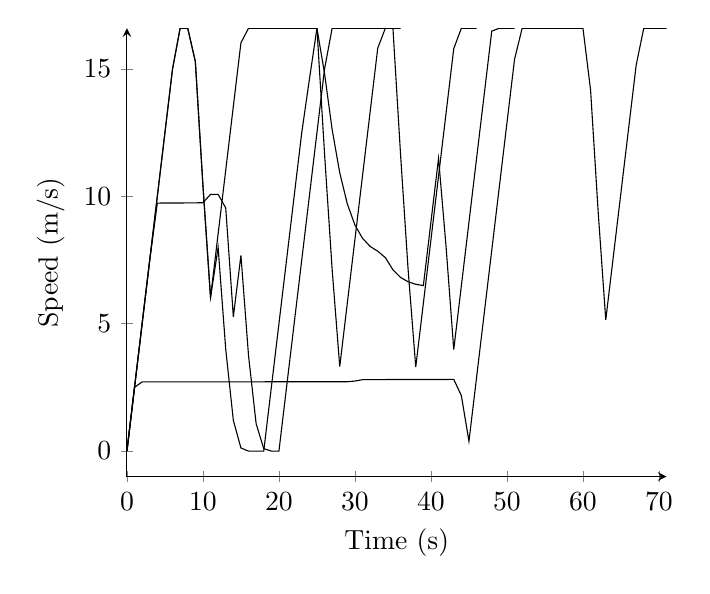
\begin{tikzpicture}
\begin{axis}[
legend style={anchor=west},
axis x line=bottom,
axis y line=left,
ymin=-1,
xlabel=Time (s),
ylabel=Speed (m/s),
]
\addplot[] coordinates {
(0, 0.0)
(1, 2.5)
(2, 5.0)
(3, 7.5)
(4, 10.0)
(5, 12.5)
(6, 15.0)
(7, 16.6)
(8, 16.6)
(9, 15.292252112)
(10, 10.4272022772)
(11, 6.03023471632)
(12, 8.53023471632)
(13, 11.0302347163)
(14, 13.5302347163)
(15, 16.0302347163)
(16, 16.6)
(17, 16.6)
(18, 16.6)
(19, 16.6)
(20, 16.6)
(21, 16.6)
(22, 16.6)
(23, 16.6)
(24, 16.6)
(25, 16.6)
(26, 11.6768906867)
(27, 7.12820536516)
(28, 3.31725880975)
(29, 5.81725880975)
(30, 8.31725880975)
(31, 10.8172588098)
(32, 13.3172588098)
(33, 15.8172588098)
(34, 16.6)
(35, 16.6)
(36, 16.6)
};
\addplot[] coordinates {
(0, 0.0)
(1, 2.5)
(2, 5.0)
(3, 7.5)
(4, 9.73626179141)
(5, 9.73710937658)
(6, 9.73822697251)
(7, 9.73974319001)
(8, 9.74187382961)
(9, 9.74500427557)
(10, 9.74988033518)
(11, 10.0759108967)
(12, 10.0776138873)
(13, 9.54543358488)
(14, 5.27454222234)
(15, 7.681403278)
(16, 3.74699729759)
(17, 1.07389487822)
(18, 0.0953466028993)
(19, 0.0)
(20, 0.0)
(21, 2.5)
(22, 5.0)
(23, 7.5)
(24, 10.0)
(25, 12.5)
(26, 15.0)
(27, 16.6)
(28, 16.6)
(29, 16.6)
(30, 16.6)
(31, 16.6)
(32, 16.6)
(33, 16.6)
(34, 16.6)
(35, 16.5966610581)
(36, 11.6479222085)
(37, 7.10244602261)
(38, 3.29756632158)
(39, 5.79756632158)
(40, 8.29756632158)
(41, 10.7975663216)
(42, 13.2975663216)
(43, 15.7975663216)
(44, 16.6)
(45, 16.6)
(46, 16.6)
};
\addplot[] coordinates {
(0, 0.0)
(1, 2.5)
(2, 5.0)
(3, 7.5)
(4, 10.0)
(5, 12.5)
(6, 15.0)
(7, 16.6)
(8, 16.6)
(9, 15.292252112)
(10, 10.4272022772)
(11, 6.03023471632)
(12, 7.99012976115)
(13, 3.9921055639)
(14, 1.20672649913)
(15, 0.120146145617)
(16, 0.0)
(17, 0.0)
(18, 0.0)
(19, 2.5)
(20, 5.0)
(21, 7.5)
(22, 10.0)
(23, 12.5)
(24, 14.5751337483)
(25, 16.6)
(26, 14.8227002511)
(27, 12.6230121114)
(28, 10.9246864421)
(29, 9.69884878224)
(30, 8.87189720583)
(31, 8.35209108489)
(32, 8.03374486144)
(33, 7.84664716231)
(34, 7.5943783841)
(35, 7.11511656743)
(36, 6.81778698594)
(37, 6.64515678955)
(38, 6.54892263145)
(39, 6.49671837799)
(40, 8.99671837799)
(41, 11.496718378)
(42, 7.98181309384)
(43, 3.98545643749)
(44, 6.48545643749)
(45, 8.98545643749)
(46, 11.4854564375)
(47, 13.9854564375)
(48, 16.4854564375)
(49, 16.6)
(50, 16.6)
(51, 16.6)
};
\addplot[] coordinates {
(0, 0.0)
(1, 2.5)
(2, 2.71810887071)
(3, 2.7181515535)
(4, 2.7181970686)
(5, 2.71824567259)
(6, 2.71829765184)
(7, 2.71835332675)
(8, 2.71841305671)
(9, 2.71847724597)
(10, 2.71854635052)
(11, 2.71862088629)
(12, 2.71870143884)
(13, 2.71878867502)
(14, 2.71888335687)
(15, 2.71898635853)
(16, 2.71909868658)
(17, 2.71922150502)
(18, 2.71935616581)
(19, 2.71950424662)
(20, 2.71966759781)
(21, 2.71984840116)
(22, 2.7200492441)
(23, 2.72027321402)
(24, 2.7205240195)
(25, 2.7208061473)
(26, 2.72112506796)
(27, 2.72148750824)
(28, 2.72190181622)
(29, 2.72237845771)
(30, 2.74853131918)
(31, 2.8021414082)
(32, 2.80748237848)
(33, 2.80758074603)
(34, 2.80769919681)
(35, 2.80784368014)
(36, 2.80802256506)
(37, 2.80824795213)
(38, 2.80853791992)
(39, 2.80892057847)
(40, 2.80944187558)
(41, 2.81018194918)
(42, 2.81129350157)
(43, 2.81310791024)
(44, 2.18067485839)
(45, 0.383991137057)
(46, 2.88399113706)
(47, 5.38399113706)
(48, 7.88399113706)
(49, 10.3839911371)
(50, 12.8839911371)
(51, 15.3839911371)
(52, 16.6)
(53, 16.6)
(54, 16.6)
(55, 16.6)
(56, 16.6)
(57, 16.6)
(58, 16.6)
(59, 16.6)
(60, 16.6)
(61, 14.1806859974)
(62, 9.39778735262)
(63, 5.1498164615)
(64, 7.6498164615)
(65, 10.1498164615)
(66, 12.6498164615)
(67, 15.1498164615)
(68, 16.6)
(69, 16.6)
(70, 16.6)
(71, 16.6)
};

\end{axis}
\end{tikzpicture}
\label{tik:speed:100:81}
\caption{100 percent diving with GSC on route $81$}
\end{figure}
